\chapter{Numerical Results}\label{ch:numeric}

%Here comparison = table and a plot

\section{Simulation}

\subsection{Convergence}


% Convergence metrics
\begin{figure}
  \centering
    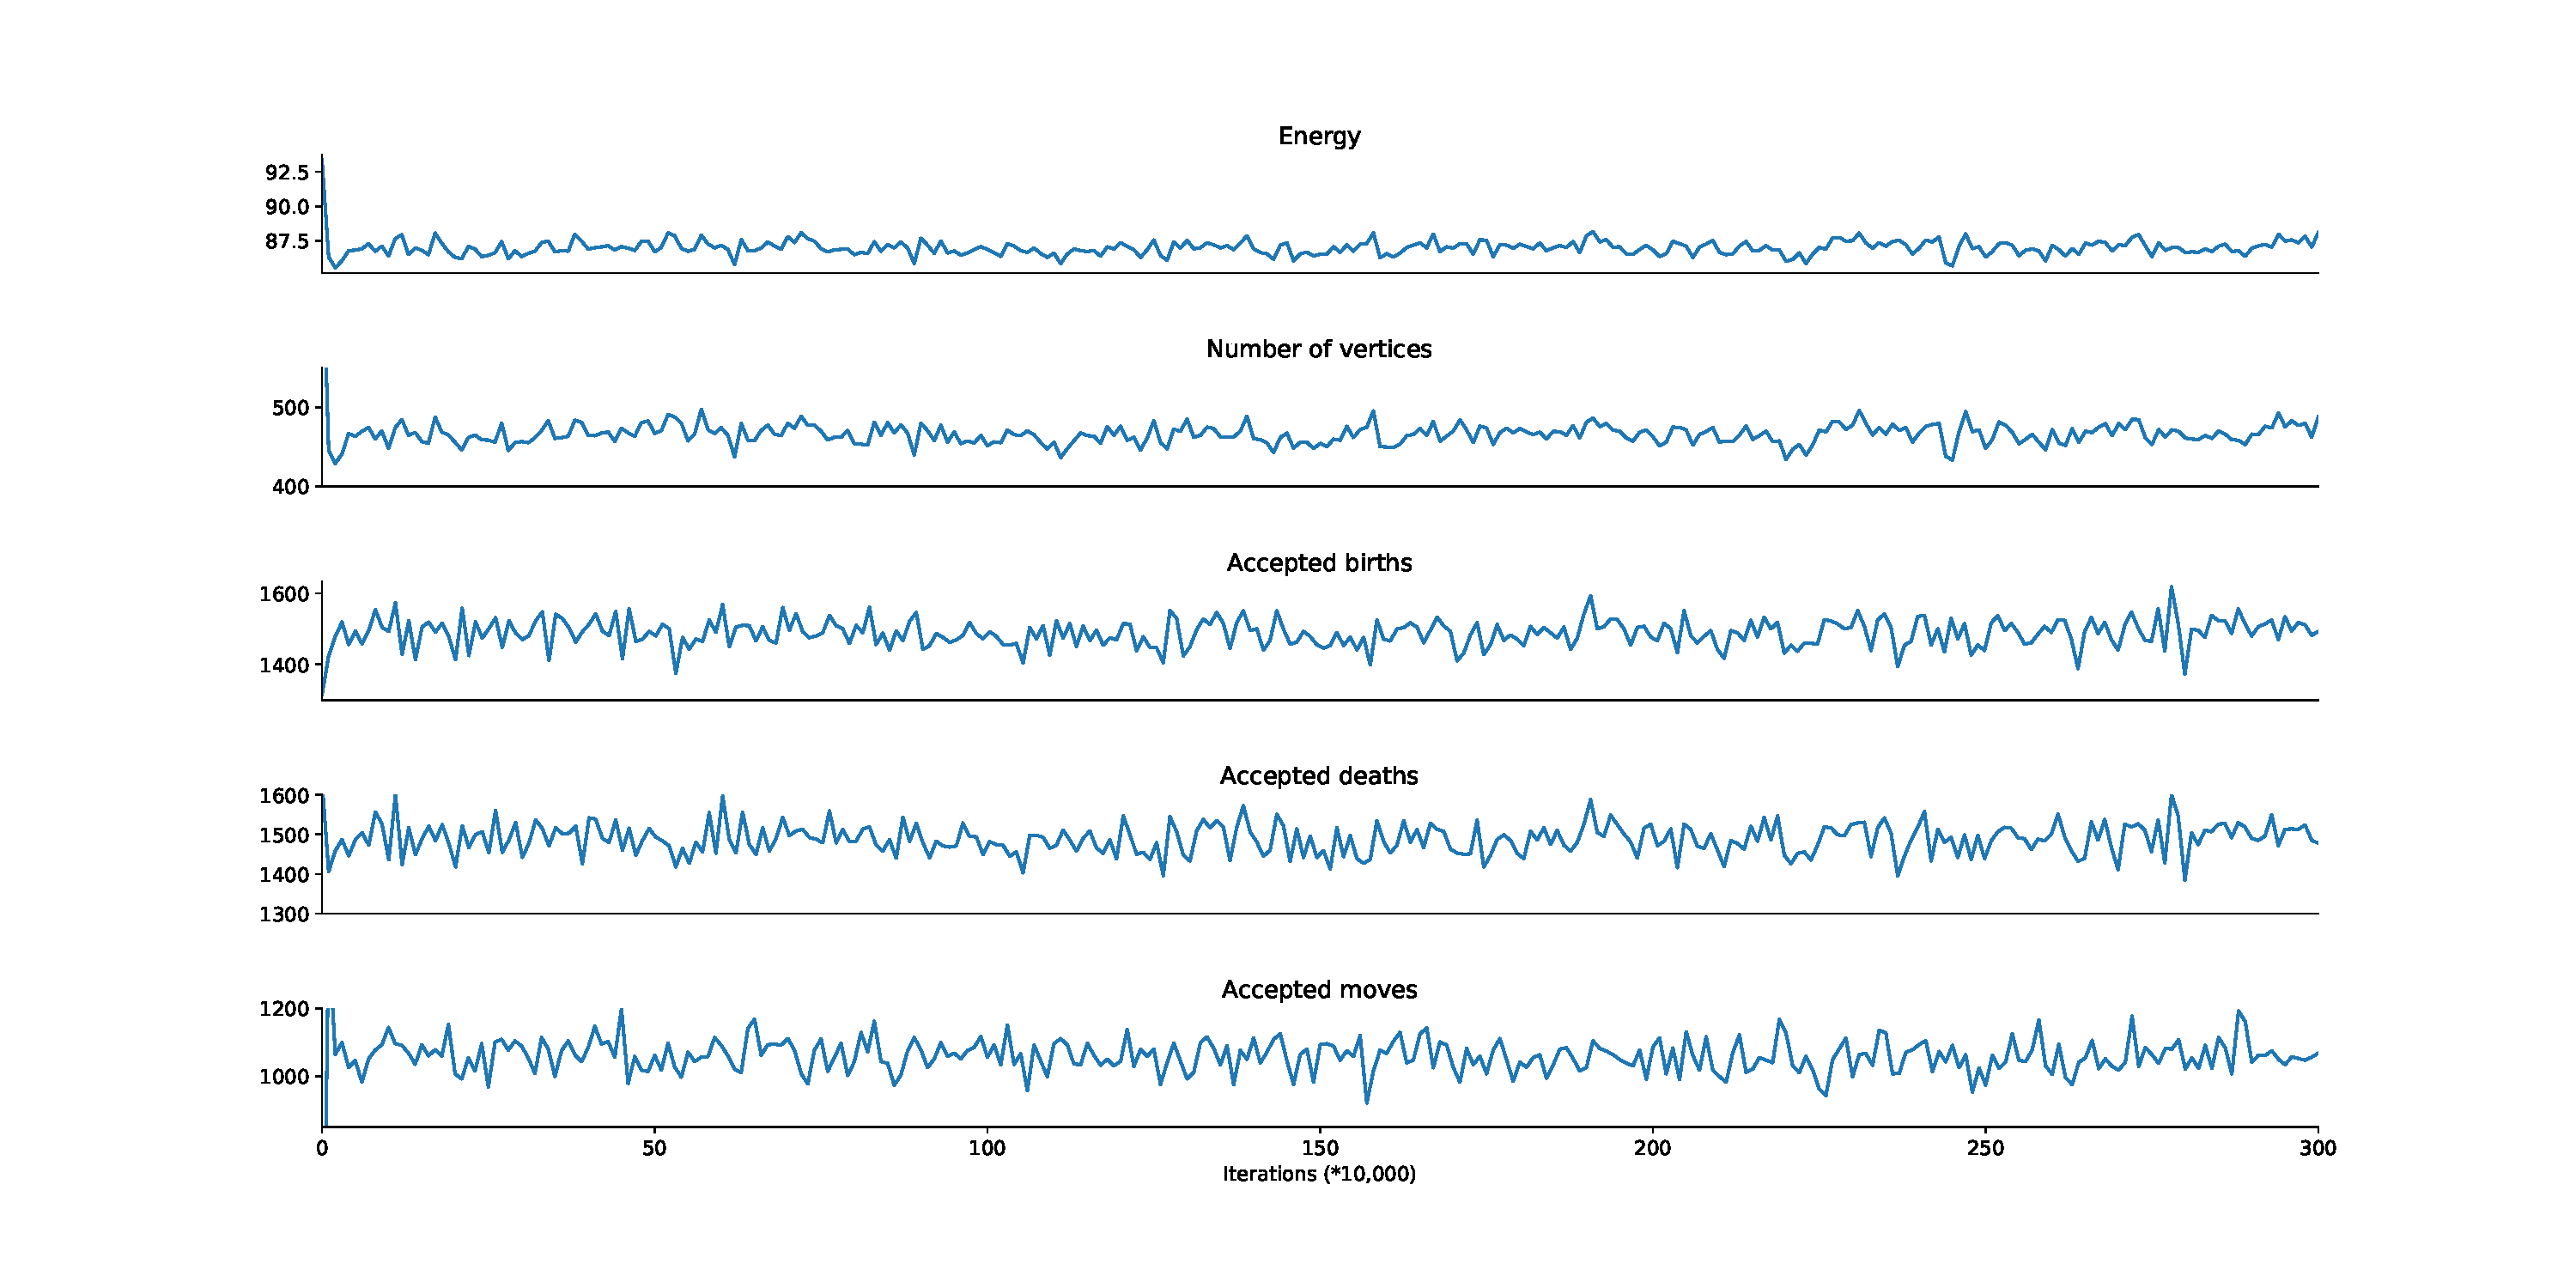
\includegraphics[width=1\textwidth]{../img/numeric/convergence.png}
  \caption{Convergence metrics. Total number of iterations: $3\times 10^6$. $\theta = 2, \alpha = 0.15, z = 500, W = 0.01$.}
\end{figure}


\todoo[inline]{Improve the convergence plot}


\subsection{Role of $\theta$}
% Plot theta low high
\todoo[inline]{Improve the theta low-high plot}

\begin{figure}
  \centering
    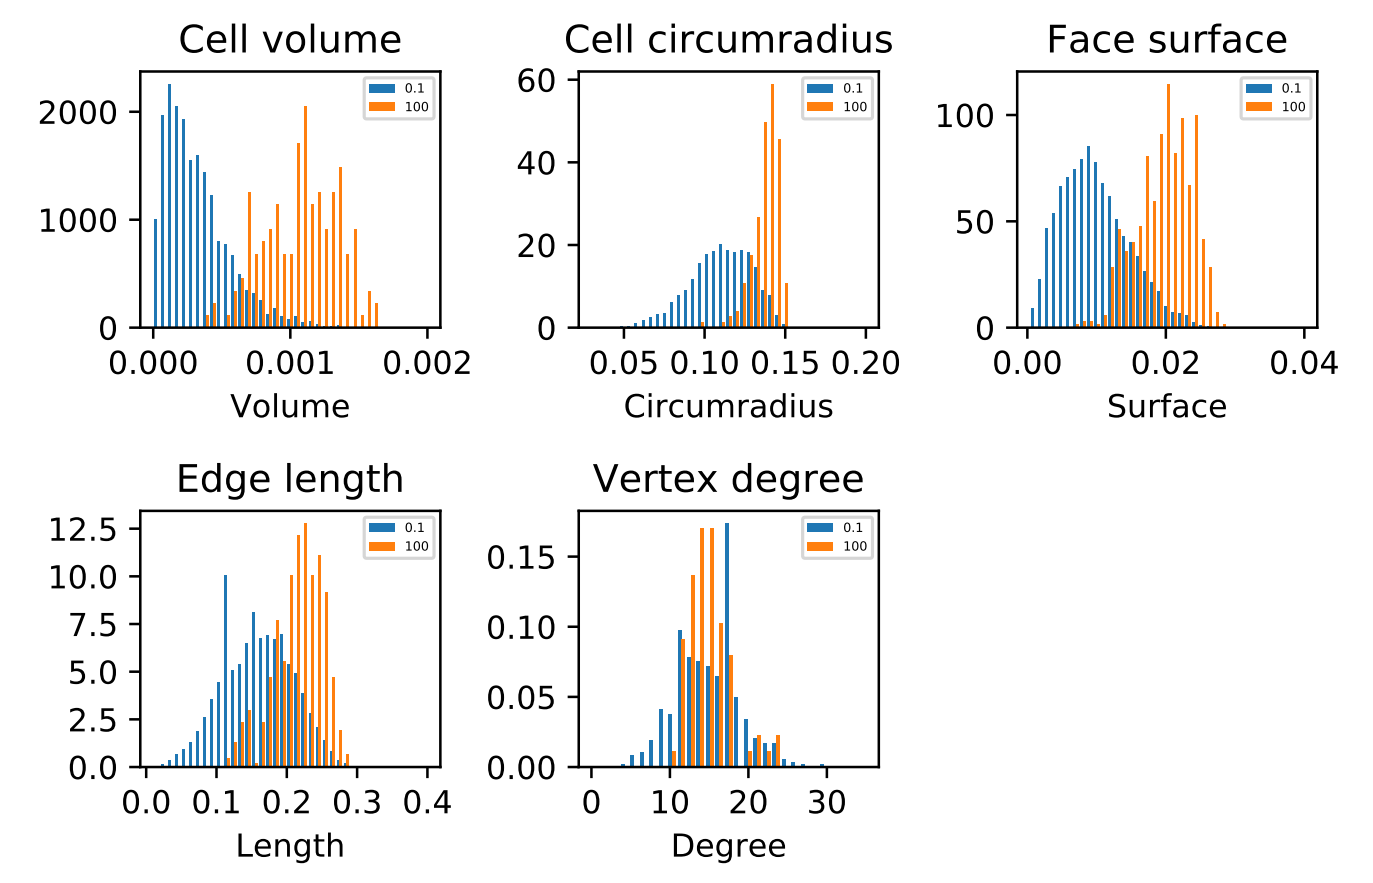
\includegraphics[width=1\textwidth]{../img/numeric/thetacomparison.png}
  \caption{Comparison of the distribution of facet statistics for one realization of \texttt{L+} model with $\alpha=0.15,z=500,W=0.01$ and $\theta = 0.01,100$.  }
\end{figure}


% Plot theta pos neg
\begin{figure}
  \centering
    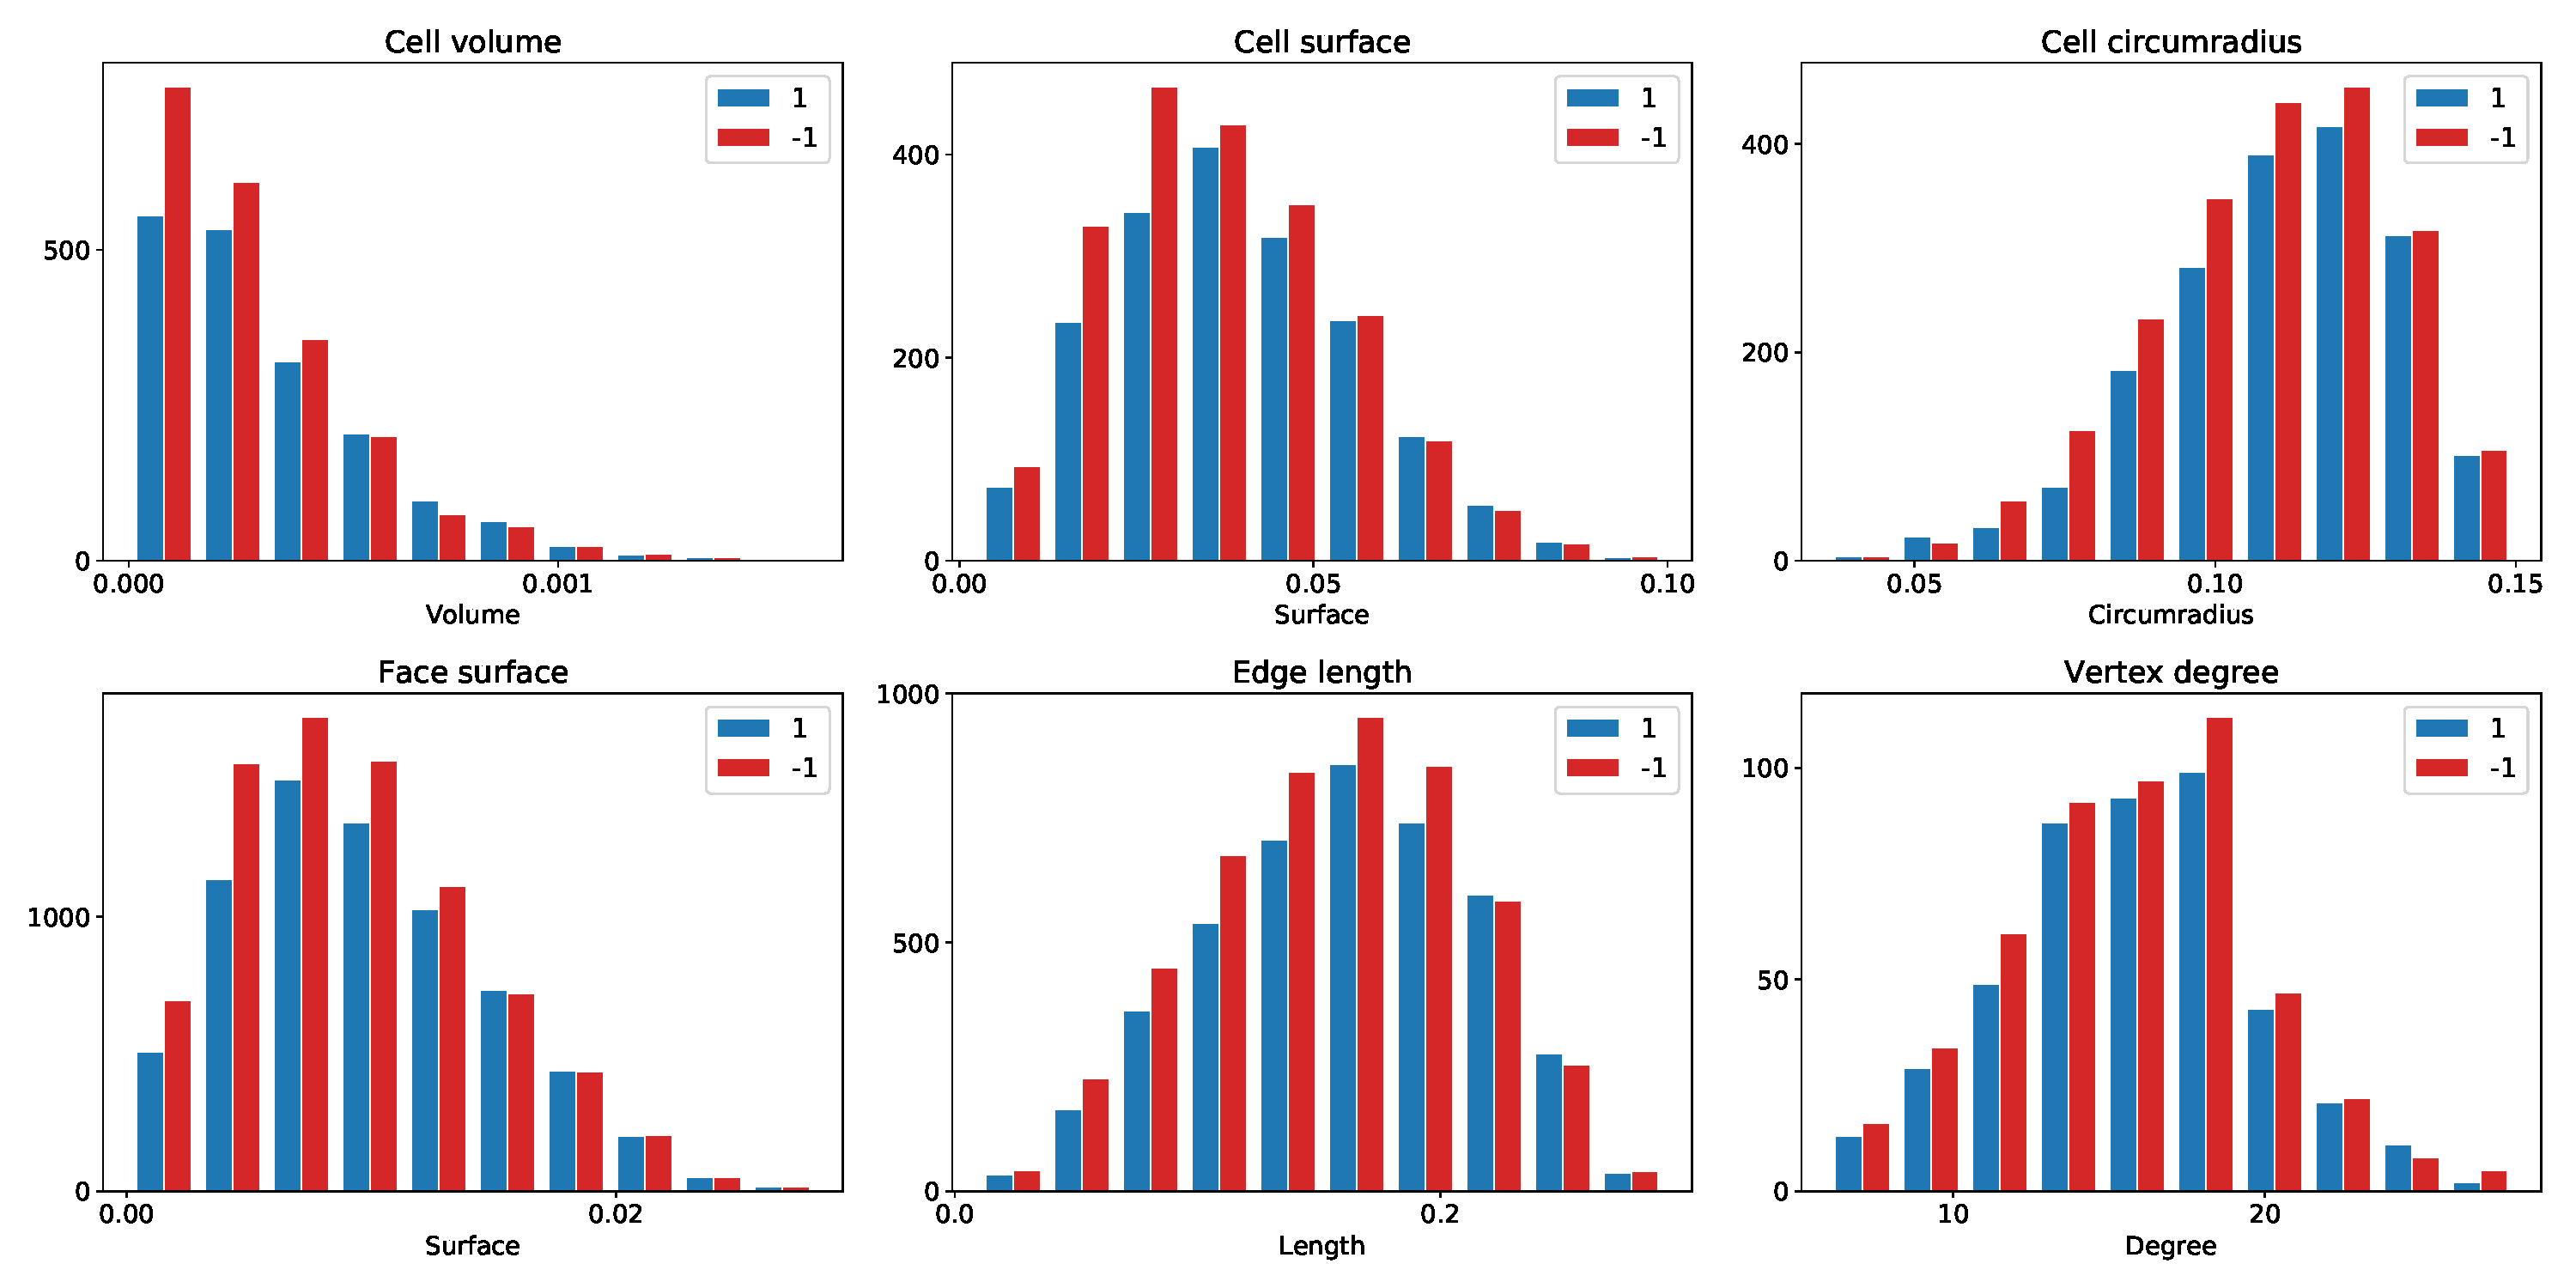
\includegraphics[width=1\textwidth]{../img/numeric/facets_1_-1.pdf}
  \caption{Comparison of the distribution of facet statistics for one realization of \texttt{L+} model with $\alpha=0.15,z=500,W=0.01$ and $\theta = -1,1$.  }
\end{figure}



\todoo[inline]{It would probably make more sense to have a table averaging over all realizations. Do that}

\begin{table*}\centering
\ra{1.3}
\begin{tabular}{lllllll}\toprule
& \multicolumn{3}{c}{Cell} & Face & Edge & Vertex \\ 
\cmidrule(lr){2-4} \cmidrule(lr){5-5} \cmidrule(lr){6-6} \cmidrule(lr){7-7}
Theta & Volume & Circumradius & Surface & Surface & Length & Degree \\
\midrule
1.0 &  0.00031 & 0.11011 & 0.03840 & 0.00963 & 0.15890 & 15.80\\
&  (0.00024) &  (0.02019) &  (0.01691) &  (0.00505) &  (0.05246) &  (3.86) \\
0.5 &  0.00033 & 0.11116 & 0.03975 & 0.00997 & 0.16157 & 15.70\\
&  (0.00025) &  (0.02010) &  (0.01739) &  (0.00521) &  (0.05395) &  (3.82) \\
-0.5 &  0.00031 & 0.11094 & 0.03882 & 0.00975 & 0.15987 & 15.65\\
&  (0.00024) &  (0.01996) &  (0.01702) &  (0.00512) &  (0.05344) &  (4.04) \\
-1.0 &  0.00028 & 0.10800 & 0.03650 & 0.00916 & 0.15570 & 15.53\\
&  (0.00022) &  (0.02033) &  (0.01609) &  (0.00486) &  (0.05220) &  (3.99) \\
\bottomrule
\end{tabular}
\caption{Facet statistics for a realization of the model $L+$ with $\alpha = 0.15, z=500, W=0.01$ with different values of $\theta$}
\end{table*}



\subsubsection{Obtaining the Poisson tetrahedrization}

% Plot theta 0.01 with Poisson theoretic
\begin{figure}
  \centering
    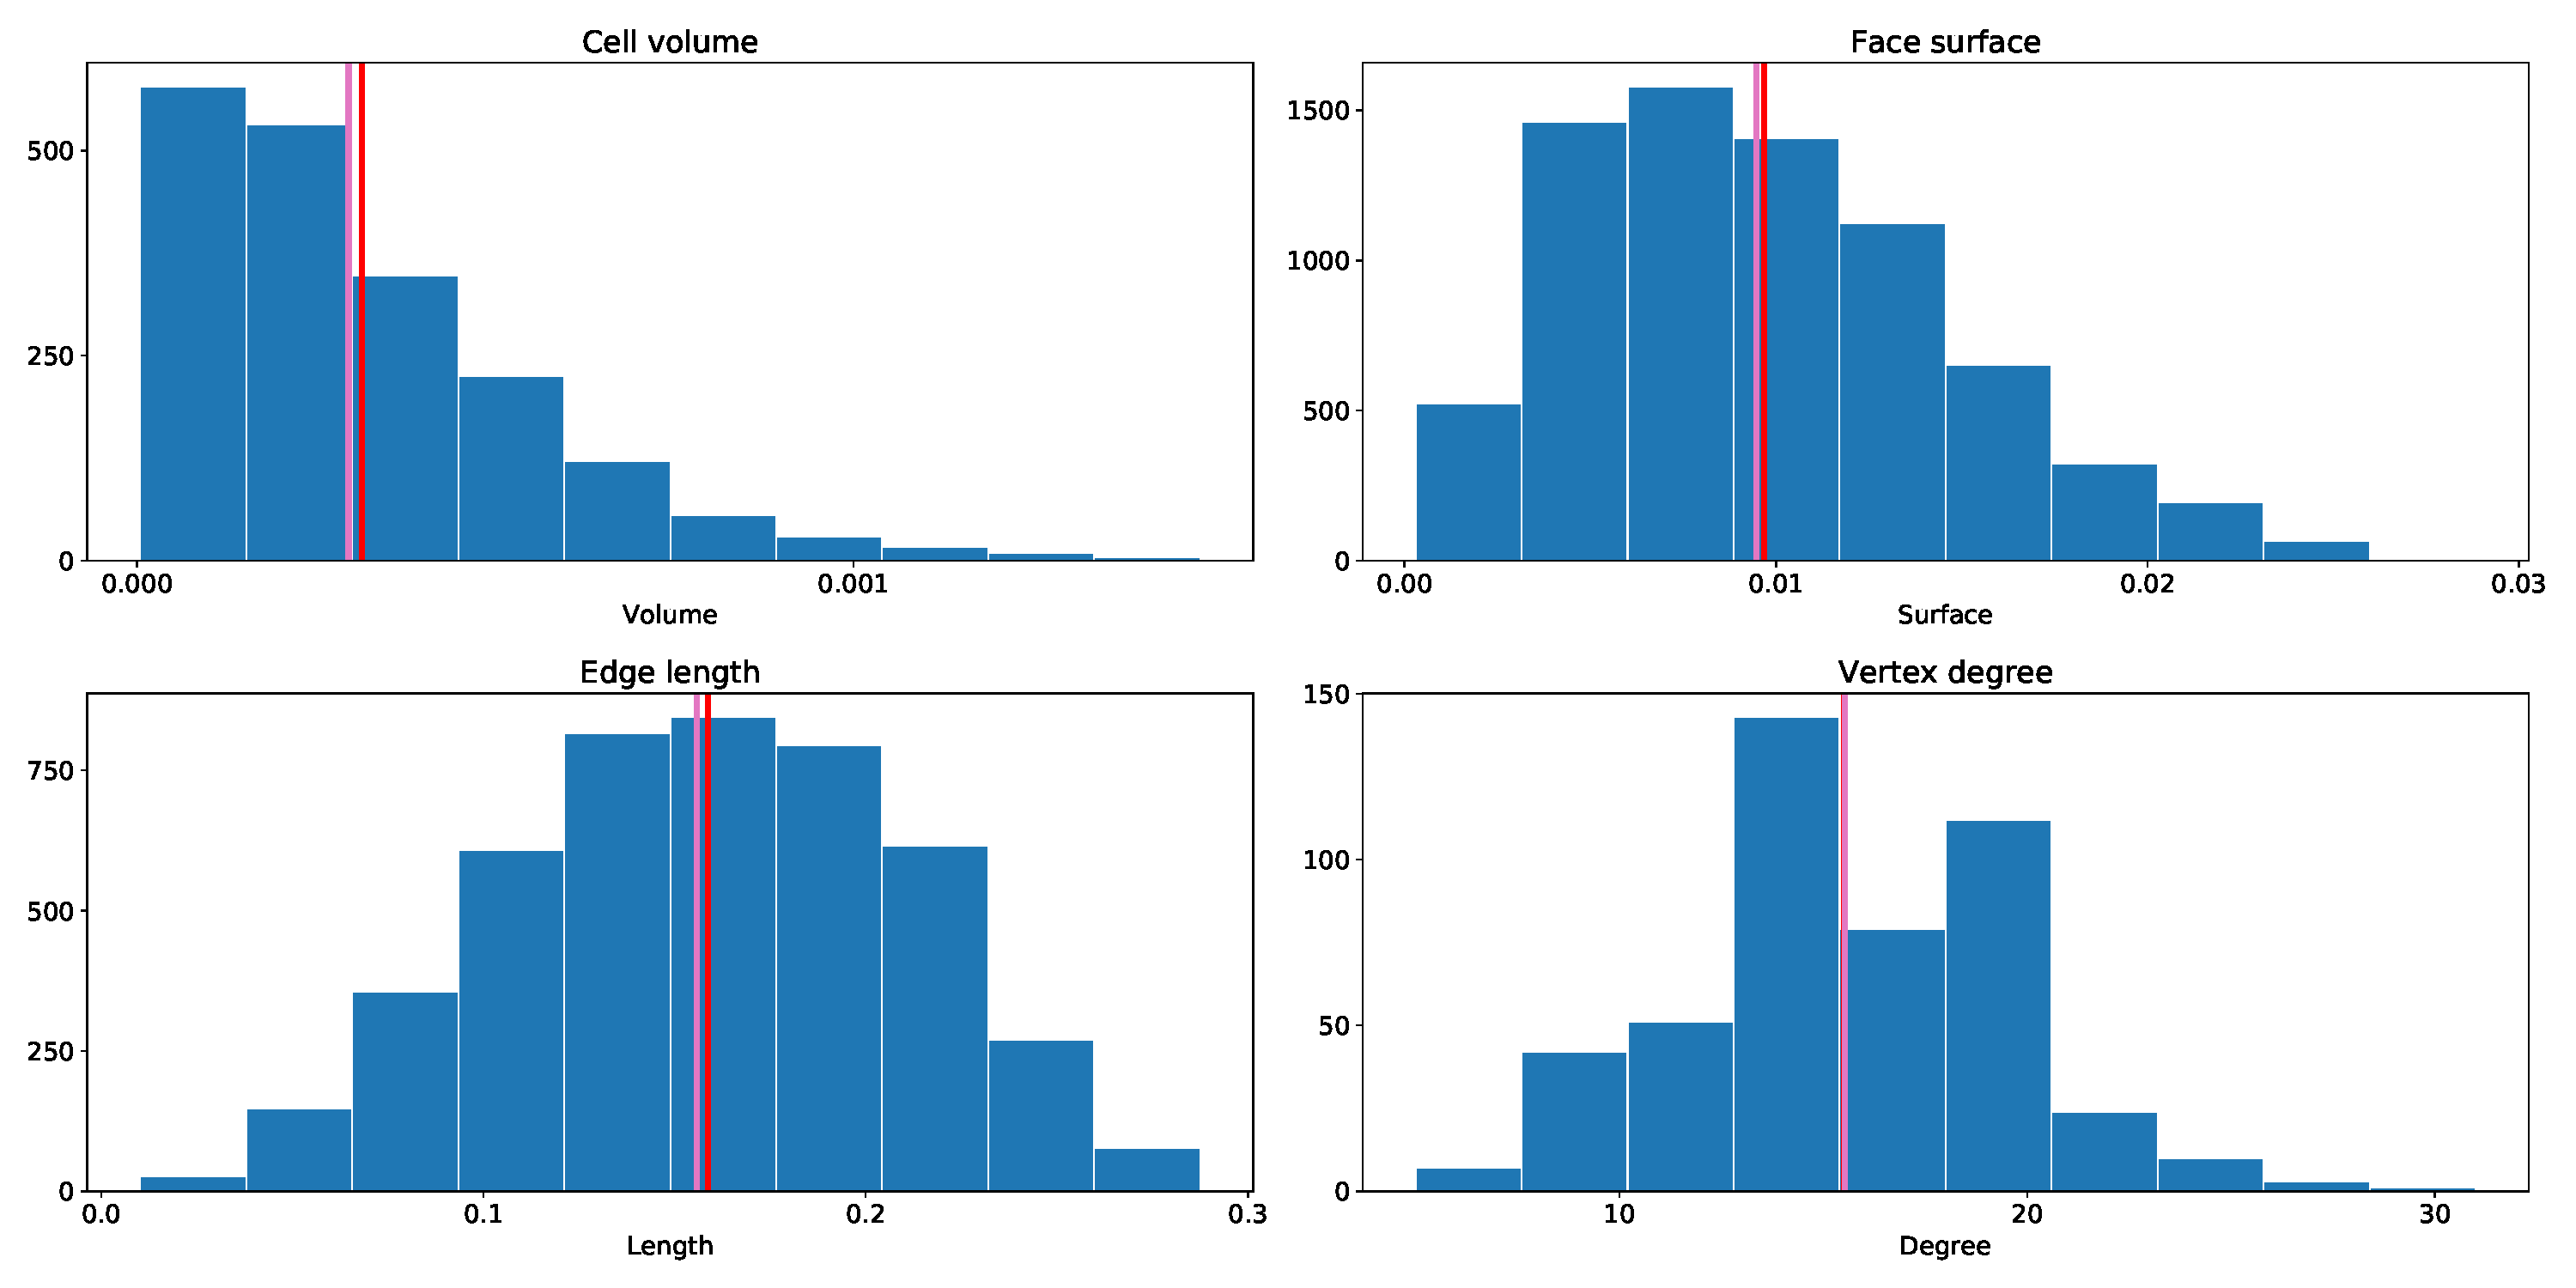
\includegraphics[width=1\textwidth]{../img/numeric/poisson.png}
  \caption{Facet distributions of a realization of the \texttt{L+} model with $\alpha=0.15,z=500,W=0.01$ and $\theta = 0.01$. Red line is the expected value for a Poisson-tetrahedrization, green line is the empirical mean of the realization.  }
\end{figure}



\todoo[inline]{Improve the poisson plot}

\subsection{Difference between Laguerre and Delaunay}


% Plot model differences 
\begin{figure}
  \centering
    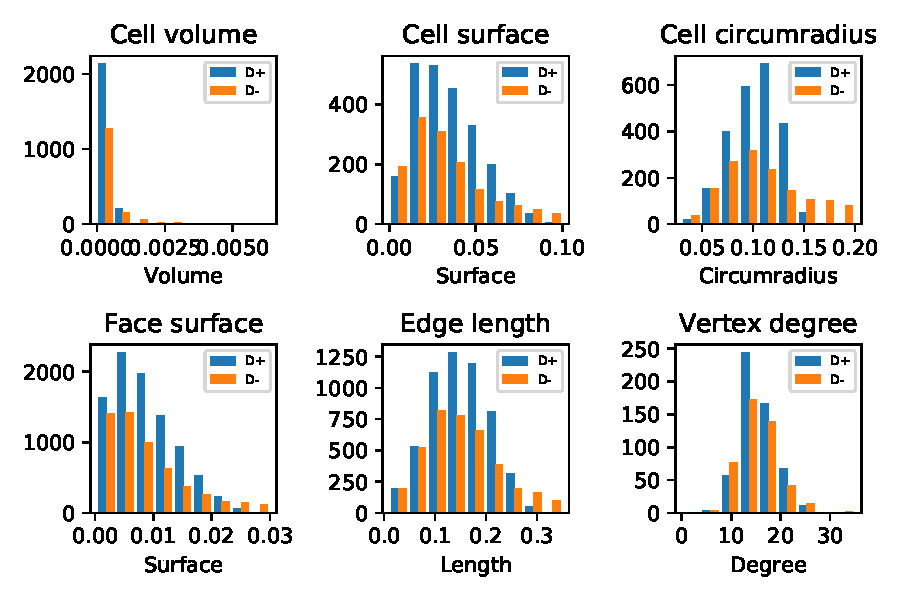
\includegraphics[width=1\textwidth]{../img/numeric/facets_D+_D-.pdf}
  \caption{Facet distribution for the models \texttt{D+} and \texttt{D-}. Parameters $\theta = 1,\alpha = 0.15, z=500, W=0.01$ for both models.}
\end{figure}

\begin{figure}
  \centering
    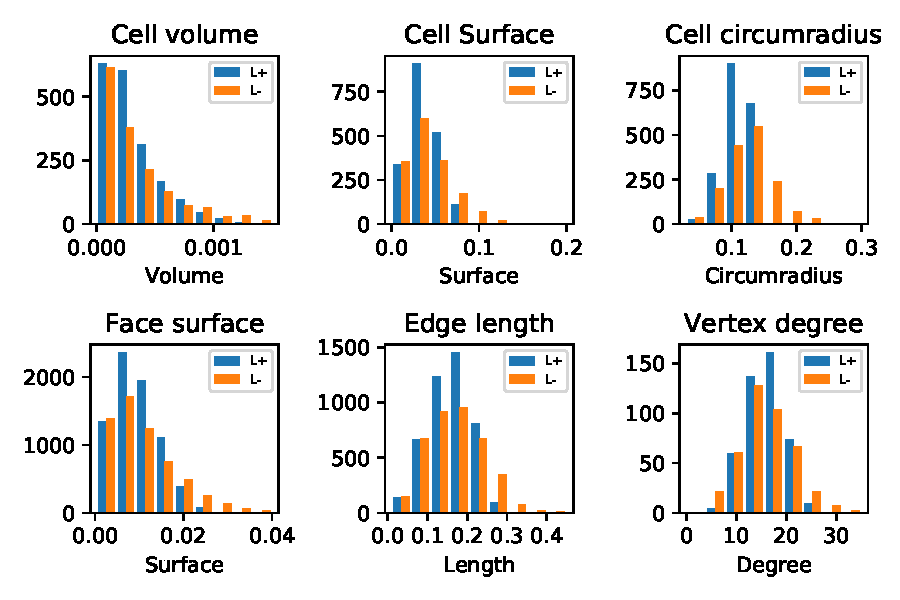
\includegraphics[width=1\textwidth]{../img/numeric/facets_L+_L-.pdf}
  \caption{Facet distribution for the models \texttt{L+} and \texttt{L-}. Parameters $\theta = 1,\alpha = 0.15, z=500, W=0.01$ for both models.}
\end{figure}

\begin{figure}
  \centering
    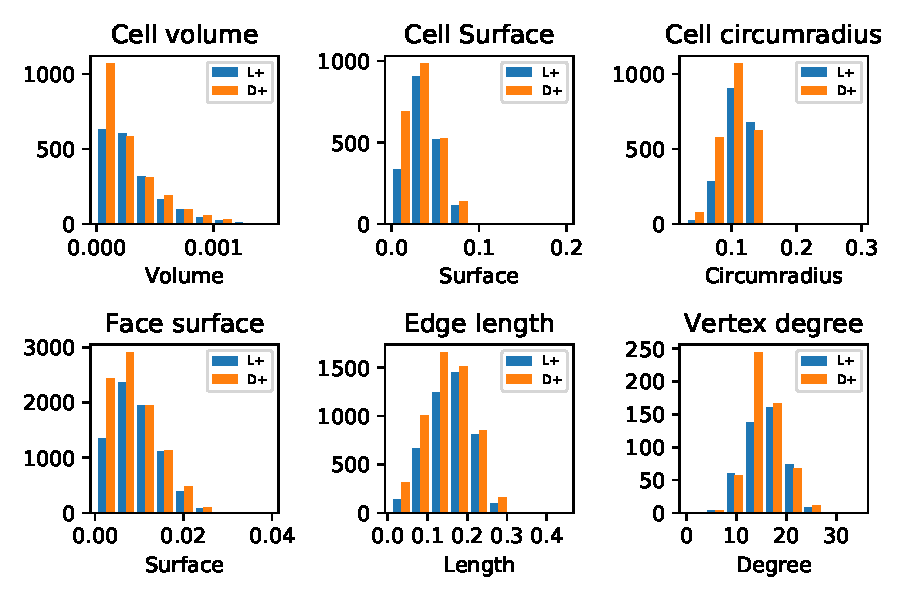
\includegraphics[width=1\textwidth]{../img/numeric/facets_L+_D+.pdf}
  \caption{Facet distribution for the models \texttt{D+} and \texttt{L+}. Parameters $\theta = 1,\alpha = 0.15, z=500, W=0.01$ for both models.}
\end{figure}


% Table model differences
\begin{table*}\centering
\ra{1.3}
\begin{tabular}{lllllll}\toprule
& \multicolumn{3}{c}{Cell} & Face & Edge & Vertex \\
\cmidrule(lr){2-4} \cmidrule(lr){5-5} \cmidrule(lr){6-6} \cmidrule(lr){7-7}
Model & Volume & Circumradius & Surface & Surface & Length & Degree \\
\midrule
D+ &  0.00027 & 0.10374 & 0.03472 & 0.00873 & 0.15033 & 15.51\\
&  (0.00024) &  (0.02323) &  (0.01827) &  (0.00535) &  (0.05644) &  (3.56) \\
D- &  0.00040 & 0.11486 & 0.04245 & 0.01066 & 0.15611 & 15.25\\
&  (0.00066) &  (0.04551) &  (0.03859) &  (0.01067) &  (0.08039) &  (4.08) \\
L+ &  0.00031 & 0.11011 & 0.03840 & 0.00963 & 0.15890 & 15.80\\
&  (0.00024) &  (0.02019) &  (0.01691) &  (0.00505) &  (0.05246) &  (3.86) \\
L- &  0.00036 & 0.12892 & 0.04326 & 0.01086 & 0.16831 & 15.76\\
&  (0.00039) &  (0.04845) &  (0.02612) &  (0.00763) &  (0.06951) &  (5.27) \\
\bottomrule
\end{tabular}
\caption{Facet statistics of one realization of each the four models. All parameters set to $\theta = 1, \alpha = 0.15, z=500, W=0.01$.}

\end{table*}

\section{Estimation}
% Estimation results (table+plot) for a few models

\begin{figure}
  \centering
    \includegraphics[width=1\textwidth]{"../img/numeric/estimation - type_D-_theta_1"}
  \caption{Estimation results for the model \texttt{D-} with parameters $\theta=1,z=500,W=0.01$ for 100 realizations.}
\end{figure}


\begin{figure}
  \centering
    \includegraphics[width=1\textwidth]{"../img/numeric/estimation - type_D+_theta_1"}
  \caption{Estimation results for the model \texttt{D+} with parameters $\theta=1,\alpha=0.15,z=500,W=0.01$ for 100 realizations. Average number of removable points: $442$.}
\end{figure}

\begin{figure}
  \centering
    \includegraphics[width=1\textwidth]{"../img/numeric/estimation - type_L-_theta_1"}
  \caption{Estimation results for the model \texttt{L-} with parameters $\theta=1,z=500,W=0.01$ for 100 realizations. }
\end{figure}


\begin{figure}
  \centering
    \includegraphics[width=1\textwidth]{"../img/numeric/estimation - type_L+_theta_1"}
  \caption{Estimation results for the model \texttt{L+} with parameters $\theta=1,\alpha=0.15,z=500,W=0.01$ for 100 realizations. Average number of removable points: $261$.}
\end{figure}
